\section{Sequential Pattern Mining}

In this section we performed sequential pattern mining following 2 approaches. 
In the first approach, we used all the tracks produced by the Hip-Hop singer:"The Impossebulls". In total we worked with 68 tracks, each of which with a length of 657 time stamps. 
In the pre-processing step, we converted each time series into sequences. 
We first applied a SAX approximation using 60 segments and 20 symbols.
At the end of this step each track was represented as an numpy array of size 60. However we noticed that our tracks were represented by sequences of 1 transaction of 60 events each. Clearly this transformation lost the concept of time. In order to recover that, we split each sequence into 30 transactions of 2 events each. This enabled us to discover frequent sequences over a span time of 30 transactions per sequence.
Below we graphically summarize the transformation adopted.

\begin{table}[htb!]
\begin{tabular}{l}
\textbf{\begin{tabular}[c]{@{}l@{}}Original sequence obtained using SAX tranform (20 symbols, 60 segments)\\ Sequence of 1 transaction with 60 events.\end{tabular}}                                                                                                                                     \\
\begin{tabular}[c]{@{}l@{}}{[} 16,  4,  9, 13, 10, 15, 10, 11,  9, 10, 19,  5,  6, 15, 11,  8,  8, 10,  9,  9, 17,  6,  2, 13,  5, 15, 11, 12,  6,  9, 17, 11,\\  5,  6,  9,  4,  9, 15,  7,  8, 14,  9, 11,  8,  8, 10,  7, 14,  8,  7,  9, 4,  3,  5,  9,  1,  3, 11,  9, 11 {]}\end{tabular}        \\
\textbf{Transformed: Sequence of 30 transactions with 2 events each.}                                                                                                                                                          \\
\begin{tabular}[c]{@{}l@{}}{[} (16, 4), (9, 13), (10, 15), (10, 11), (9, 10), (19, 5), (6, 15), (11, 8), (8, 10), (9, 9), (17, 6), (2, 13), (5, 15),\\ (11, 12), (6, 9), (17, 11), (5, 6), (9, 4), (9, 15), (7, 8), (14, 9), (11, 8), (8, 10), (7, 14), (8, 7), (9, 4), (3, 5),\\ (9, 1), (3, 11), (9, 11) {]}\end{tabular}
\end{tabular}
\end{table}

We then extracted frequent sequences using prefixspan with a min support of 18\%. In Table 5.1 we show the top 5 frequent sequences that were obtained. It's worth to mention that the explainability of the results was limited by the approximation applied to the time series.
As a second approach instead, we used the information provided by the features "tags" and "date\_created", which were obtained from the dataset tracks.csv. Selecting tracks belonging to one single artist we could explore how the tags associated with the song of that artist changed over time. The dataset was composed by 266 sequences (tracks) of the singer Ars Sonor, span over a time period that goes from 2013 to 2015. After a pre-processing step, through which we converted each row into a sequence, we extracted the top 5 frequent sequences (as shown in Table 5.1). 
\begin{table}[htb!]
\centering
\begin{tabular}{ccllcc}
\cline{1-2} \cline{5-6}
\textbf{\begin{tabular}[c]{@{}c@{}}Frequent sequences\\ (spectral centroid)\end{tabular}} & \textbf{Matches} &  &  & \textbf{\begin{tabular}[c]{@{}c@{}}Frequent sequences\\ (Ars Sonors' tags)\end{tabular}} & \textbf{Matches} \\ \cline{1-2} \cline{5-6} 
{[}(7, 8){]}                                                                              & 728              &  &  & {[}('24-bit'){]}                                                                         & 176              \\ \cline{1-2} \cline{5-6} 
{[}(8, 7){]}                                                                              & 743              &  &  & {[}('era 3b'){]}                                                                         & 117              \\ \cline{1-2} \cline{5-6} 
{[}(6, 6){]}                                                                              & 723              &  &  & {[}('era 3b'), ('24-bit'){]}                                                             & 91               \\ \cline{1-2} \cline{5-6} 
{[}(7, 7){]}                                                                              & 726              &  &  & {[}('kristin e'){]}                                                                      & 41               \\ \cline{1-2} \cline{5-6} 
{[}(8, 6){]}                                                                              & 727              &  &  & {[}('wallenberg', '24-bit'){]}                                                           & 33               \\ \cline{1-2} \cline{5-6} 
\end{tabular}
\caption{Frequent sequences of spectral centroid time series (on the left) and songs' tags (on the right)}
\label{tab:my-table}
\end{table}

\section{OPTICS}

\begin{wrapfigure}{l}{.35\textwidth}
  \centering
    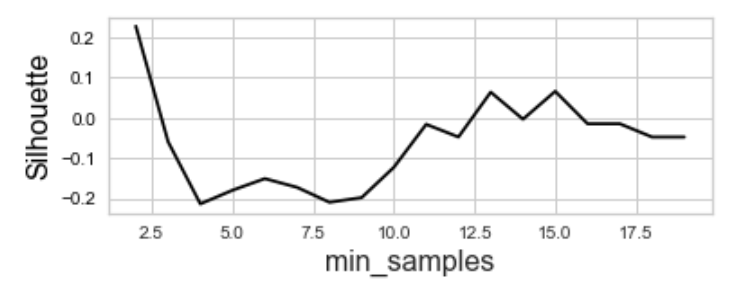
\includegraphics[width=.3\textwidth]{images/OPTICS sil.png}
  \caption{Silhouette by varying min\_samples}
\end{wrapfigure}
For this task we decided to cluster Classical songs using both OPTICS and DBSCAN, in such a way that the differences emerging from the two algorithms could be compared. In order to better study the effects of OPTICS, we decided to filter our dataset and consider only 2 features, namely: "liveness" and "danceability". This choice is driven by the fact that density based algorithm lose their effectiveness in high dimensions, and since we wanted to compare the results of the two algorithms we decided to use only a restricted by meaningful set of features. The dataset is composed by 265 tracks, whose attributes were normalized before being used in the clustering. Although OPTICS reduces the number of hyper-parameters (as we don't need to specify the epsilon radius), it still needs the setting of the parameter min\_samples, which appears to be crucial for a correct clustering. To choose the correct configuration, we plot the silhouette score by varying the number of the previously mentioned parameter (as shown in Figure 5.1). We noticed that when the min\_samples is set to 13 the silhouette is optimal (approximately 0.063). 


\begin{figure}[!htb]
  \centering
  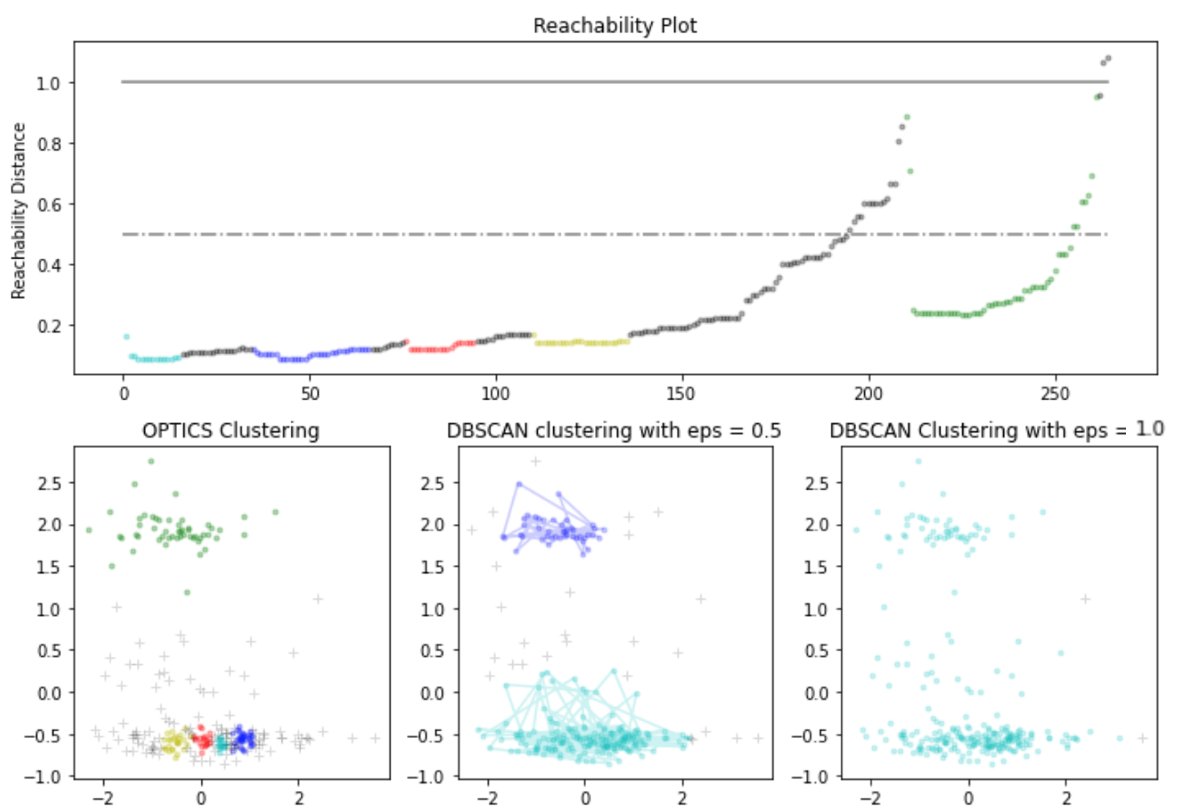
\includegraphics[width=0.8\linewidth]{images/OPTICS-Classical.png}
  \caption{OPTICS clustering compared to DBSCAN.}
\end{figure}

In Figure 5.2 we show the results obtained using OPTICS and DBSCAN. The latter was used first with a small epsilon (0.5) and then with a large one (1.0) in order to see how the clustering changed in the 2 extreme cases.
We noticed that OPTICS was able to generate 5 clusters. The green cluster (top left corner) identifies songs that are highly danceable and that were not recorded during live concerts. We notice that majority of classical songs are not suitable for dancing, as the remaining 4 clusters have low danceability regardless of the liveness coefficient. It is interesting to see that while the green cluster was detected also using DBSCAN, the latter grouped the 4 clusters identified by OPTICS in one single cluster. This highlights the difficulties that DBSCAN faces when clusters with different density are close to each other. OPTICS on the other hand, performed well in the task of differentiating clusters in area with heterogeneous density.
On the reacheability graph, the dot line represents the cut off level after which data points are considered outlier in DBSCAN with epsilon = 0.5, while the straight line has the same meaning w.r.t. DBSCAN with epsilon = 1. 

\section{Transactional Clustering: K-Modes}

For this task we used a dataset built with discretized continuous features extracted from echonest.csv and categorical attributes obtained from tracks.csv (from this dataset we used: language, license and genre). For discretizing the continuous variables, we processed each attribute and identified the best threshold for generating the categorical values. Below we summarize the results. 

\begin{table}[htb!]
\centering
\begin{tabular}{ll}
\hline
\textit{\textbf{Features}} & \textit{\textbf{Discrete values}}           \\ \hline
\textbf{Energy}            & {[}'low', 'medium', 'high'{]}               \\ \hline
\textbf{Emotions}           & {[}'sad', 'happy'{]}                        \\ \hline
\textbf{Liveness}          & {[}'recorded live', 'recorded in studio'{]} \\ \hline
\textbf{Speechiness}       & '{[}instrumental', 'balanced', 'spoken'{]}  \\ \hline
\textbf{Danceability}      & {[}'not danceable', 'danceable'{]}          \\ \hline
\textbf{Listens}           & {[}'low', 'medium', 'high'{]}               \\ \hline
\end{tabular}
\caption{Continuous variable discretized for K-Modes algorithm.}
\label{tab:my-table}
\end{table}

In total the transactional dataset has 9 features and 4784 instances.
To determine the optimal number of clusters, we performed several trials and we selected the one with the most interesting results.
We clustered the data with K=3 using Huang initialization repeated 50 times. Below we show the centroids yielded by the K-Modes algorithm.


\begin{table}[htb!]
\centering
\begin{tabular}{cl}
\hline
\textbf{Clusters} & \multicolumn{1}{c}{\textbf{Centroids}}                                                                                                                                                                                                                  \\ \hline
\textbf{0}        & \begin{tabular}[c]{@{}l@{}}{[} language: 'English',  'low\_listens', 'Rock', 'danceable', energy: 'medium',\\  license: 'Attribution-Noncommercial-Share Alike 3.0 United States' ,\\ 'instrumental', 'happy',  'recorded\_in\_studio' {]}\end{tabular} \\ \hline
\textbf{1}        & \begin{tabular}[c]{@{}l@{}}{[} language: 'English', 'low\_listens', 'Folk', 'not\_danceable', energy: 'low', \\ license: 'Attribution-Noncommercial-Share Alike 3.0 United States',\\ 'recorded\_in\_studio', 'instrumental', 'sad' {]}\end{tabular}    \\ \hline
\textbf{2}        & \begin{tabular}[c]{@{}l@{}}{[} language: 'English', 'low\_listens', 'Rock', 'not\_danceable', energy: 'high',\\  license: 'Attribution-Noncommercial-Share Alike 3.0 United States',\\ 'recorded\_in\_studio', 'instrumental', 'sad' {]}\end{tabular}   \\ \hline
\end{tabular}
\caption{K-Modes centroids.}
\label{tab:my-table}
\end{table}

We noticed that we obtained 2 centroids in which the genre Rock is present. One of which (cluster 0) groups songs which are considered happy, danceable and having medium energy, while the other centroid (of cluster 2) represent sad songs which strangely have high energy and are not danceable. 
The most interesting centroid is the 2nd, which is representative of sad Folk songs. Tacks in this cluster, are not danceable since they have low energy. We concluded that this cluster grouped relaxing songs that stimulate melancholic and sad emotions.
To better visualize and understand the composition of the obtained clusters we built and inspected the related count-plot. Below we show only the most significant ones.

\begin{figure}[!htb]
  \centering
  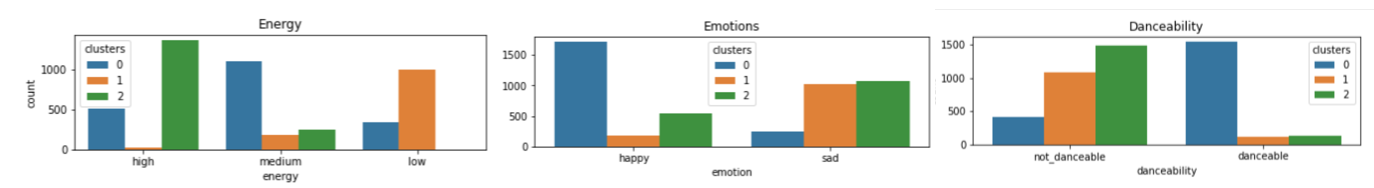
\includegraphics[width=1\linewidth]{images/transactional_clustering.png}
  \caption{Count-plots of Energy, Danceability and Emotions}
\end{figure}

\section{AI Explainability: LIME}
In this section we extracted an explanation that provided the reasons why the Random Forest classifier described in the previous sections, classifying the test instances in certain way.
To do so, we first built and trained a Random Forest classifier using the same parameters and partitions employed in Section 3.7.1.\\ We then used LIME algorithm, which uses a logistic regression to explain the behaviour of the black box of our classifier. 
We displayed the explanation for 2 randomly selected instances (correctly classified by the model) belonging to the 2 test classes. 
\\
\\

\begin{figure}[htb!]
  \centering
  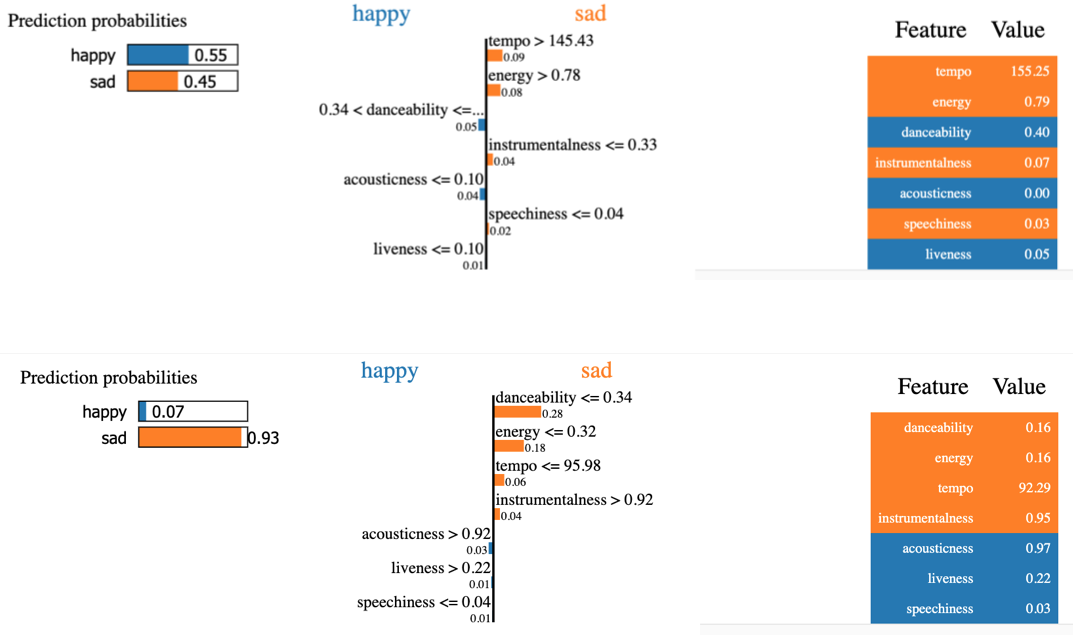
\includegraphics[width=1\linewidth]{images/LIME.png}
  \caption{LIME explanation of randomly sampled instances of class "sad" and class "happy".}
\end{figure}

The explainer of instance classified as "happy" shows that the main factors that positively contributed to the result are danceability which is 0.40 (apparently a danceability $>$= 0.34 brings the classification closer to "sad" songs), tempo and energy which is 0.79.
If we compare the two explainations, we see that when energy, danceability and tempo are low, and acousticness is high ($>$0.92) the songs are identified as sad songs by the model. Instead happy songs, are characterized by high danceability, energy ($>$0.78) tempo, and low acoustincness ($<$=0.10).
\newpage